\chapter{Datos obtenidos}

En este capítulo vamos a describir los datos obtenidos a través del framework. Tuvimos algunos problemas al recolectar los audios. El principal problema fue que el ambiente utilizado por cada hablante no estaba completamente en silencio como para hacer una buena grabación. Muchos errores surgieron en esa dirección. Otros errores comunes pero no tan frecuentes fueron: interpretaciones erróneas de la consigna, errores de volumen del micrófono y saturación. 

\subsection{Mediciones}

Se realizó una clasificación manual de las grabaciones para determinar si las mismas se realizaron correctamente. Esta clasificación se realizó a  través de la herramienta de administración que vimos en el capítulo 3. Las clases que utilizamos fueron: ``Conservar’’, ``Sonido saturado’’, ``Mucho ruido de fondo’’, ``Problema en el habla’’. Esta clasificación fue empírica, o sea no realizando ningún análisis sino que escuchando manualmente cada una. La cantidad de cada clase fue la siguiente:

\begin{table}[h]
\centering
\begin{tabular}{|l|c|c|c|c|}
\hline
\textbf{}  & \textbf{Bs.As. } & \textbf{Cba.} & \textbf{Total} \\ \hline
\textbf{Conservar}  & 222 & 105 & 327 \\ \hline
\textbf{Problemas en el habla}  & 33 & 15 & 48 \\ \hline
\textbf{Mucho ruido de fondo}  & 2 & 12 & 14 \\ \hline
\textbf{Sonido saturado}  & 2 & 0 & 2 \\ \hline
\end{tabular}
\end{table}

Los datos obtenidos están desbalanceados. No fue posible obtener la misma cantidad de audios para los dos grupos. Esto se va a reflejar en la clasificación y en el análisis posterior.

\subsection{Errores comunes}

Las categorías establecidas anteriormente describen los errores comunes más frecuentes. Podemos observar que del total de 391 grabaciones, 64 tuvo algún problema. Esto representa alrededor del 16\% de los audios grabados. Es un número alto para ser un experimento guiado.

La gran causa de este número es la falta de chequeo al aceptar un audio nuevo. La detección automática de errores en el momento de grabación es un tema que excede los objetivos de esta tesis y se propone como trabajo futuro.

El análisis que se presenta a continuación está basado en los audios clasificados como ``Conservados’’.

\section{Alineación forzada}

El alineador automático no realiza su función de forma perfecta. En ocasiones, el proceso de alineamiento forzado introduce errores. Es muy importante descartar los audios mal alineados, ya que si no cuando los procese el extractor nos darían información errónea. Fuimos chequeando cada audio etiquetado como ``Conservado’’ y analizando si la alineación fue correcta con la aplicación Praat \cite{praat}. Los errores de alineamiento más comunes se debieron a:

\begin{itemize}
    \item \textbf{Ruido de fondo:} los audios donde el alineador se comporta de peor manera son aquellos en los que se escucha ruido de fondo. En esos casos, las alineaciones resultan muy malas. Lamentablemente en nuestro caso esto es bastante común. En la Fig. \ref{alinMala} se puede ver un ejemplo utilizando Praat.

\begin{figure}[h!]
    \centerline{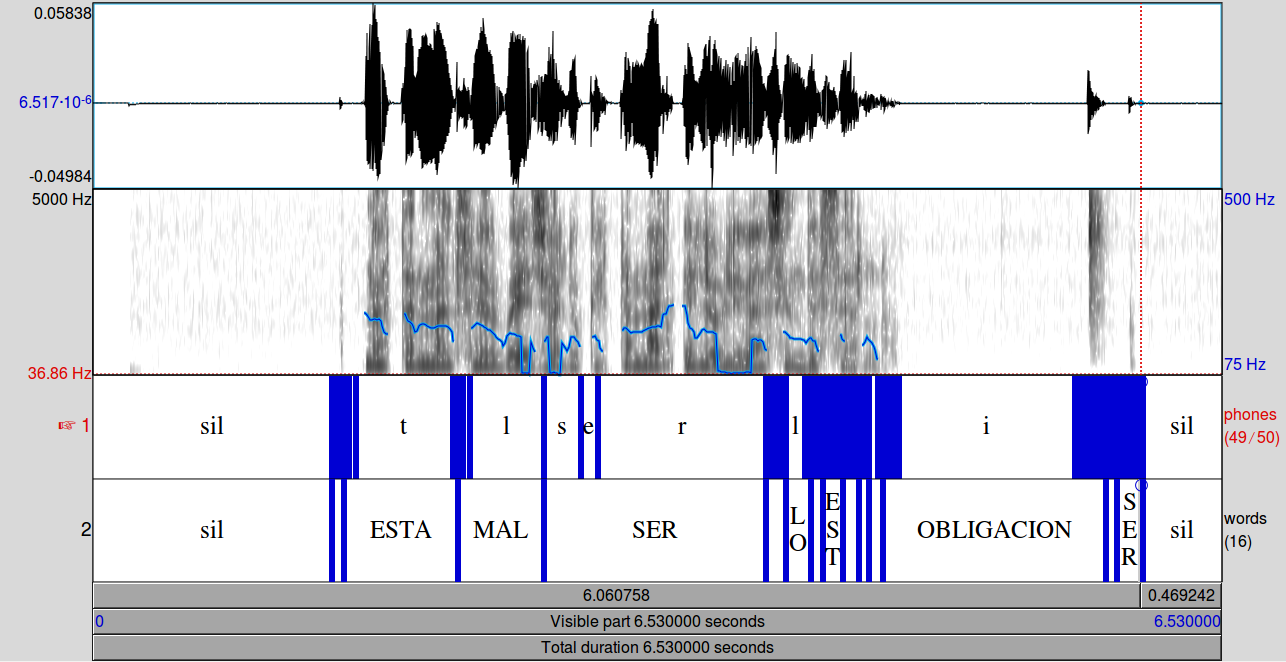
\includegraphics[width=0.8\textwidth]{alineacion_mala_inf} }
    \caption{Ejemplo de alineación mala por ruido}
    \label{alinMala}
\end{figure}

    \item \textbf{Mouse clic al finalizar:} las grabaciones recibieron muchos ruidos del ambiente. Pasó en muchas oportunidades que el clic de finalizar del mouse se grabó como parte final en el audio (Ver Fig. \ref{clickFinal}). Ese sonido se grabó y afectó la alineación de forma tal que el alineador lo confunde como habla.
    
\begin{figure}[h!]
    \centerline{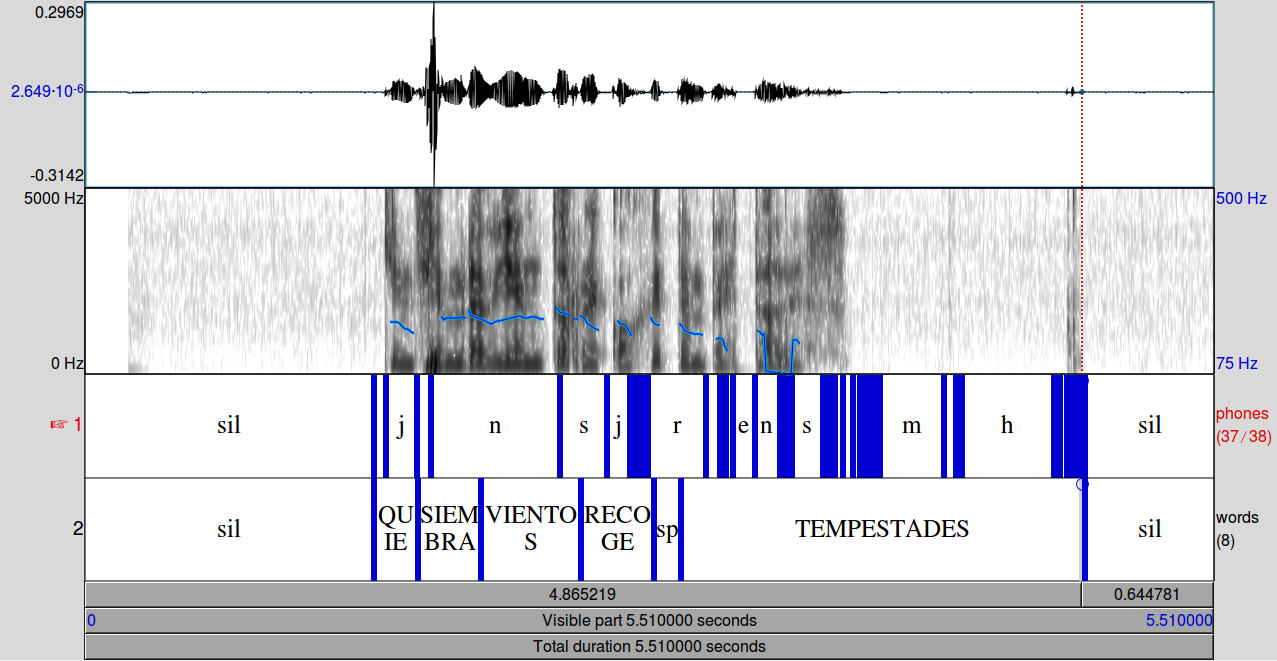
\includegraphics[width=0.8\textwidth]{click_al_final_inf} }
    \caption{Clic al final}
    \label{clickFinal}
\end{figure}

    \item \textbf{Saturación del micrófono:} el volumen del micrófono es configurado por el hablante. Es por ello que debemos confiar en su buena voluntad. Muchas veces la grabación fue buena pero al final tuvo una entonación mucho más fuerte que las demás, haciendo que, posteriormente, la alineación no sea precisa.

    \item \textbf{Entonación exagerada:} en algunas grabaciones se quiso exagerar la entonación. Por ejemplo, las palabras finalizadas en /s/ fueron grabadas en muchos casos sosteniendo ese fonema por tiempo prolongado de forma exagerada. En la mayoría de los audios no sucedió, por lo que no afectó el análisis del experimento. El problema que surgió en estos casos fue que el hablante no supo pronunciar la frase de la forma más natural posible. 
    
\end{itemize}

\section{Corrección de errores}

%TODO: Corregir y explicar bien para qe se entiende la opcion de SCORES acá y en el capitulo anterior - leer bien el mail de prosodylab
Para corregir los errores descriptos debimos chequear cada uno de los TextGrids. Esta forma se realizó ya que eran pocos audios pero en un experimento con más hablantes se debe utilizar la opción de ``.SCORES’’ descripta en el capítulo anterior. Los resultados de la cantidad de alineamientos corregidos son:

\begin{table}[h]
\centering
\begin{tabular}{|l|c|c|c|c|}
\hline
\textbf{}  & \textbf{Bs.As. } & \textbf{Cba.} & \textbf{Total} \\ \hline
\textbf{Modificados}  & 101 & 88 & 189 \\ \hline
\textbf{Correctos sin modificación}  & 119 & 2 & 121 \\ \hline
\textbf{Total} & 220 & 90 & 310 \\ \hline
\end{tabular}
\end{table}

%TODO: acordarse porque acá tengo 310 audios y no se corresponde con los 327 que son el total de conservados.
Entonces las grabaciones que utilizamos salierond de estas 310 alineaciones. 

Recordemos que cada hablante tenía la posibilidad de grabar varias veces la misma frase con la idea de que la última grabación sea la mejor grabada. Debemos quitar estos casos para no favorecer a las frases repetidas mas que a las frase grabadas una sola vez. Los audios repetidos, en este conjunto de 310 alineamientos, son 50. Entonces, para finalizar, quitamos las grabaciones repetidas. Las grabaciones que utilizamos para seguir realizando este análisis son 260. 

En la próxima sección veremos el análisis que realizamos con estas grabaciones. 